\documentclass[11pt,a4paper]{article}
% \usepackage[a4paper,margin=1in]{geometry}
\usepackage[a4paper,margin=2cm]{geometry}
\usepackage[utf8]{inputenc}

\title{
Cloze Deletion Prediction\\
\large LT2306/LT2316 H18
}
\author{
Stefan Eng\\
\textit{gussteen@student.gu.se}\\
Göteborgs universitet
}
\date{November 2018}

\usepackage{dirtytalk}
\usepackage{csquotes}
\usepackage{natbib}
\usepackage{graphicx}
\usepackage{url}
\usepackage{booktabs}


\begin{document}

\maketitle

\section{Introduction}
A cloze deletion test is a form of language test where a sentence (or paragraph) is given to the test taker with blanks for missing words \cite{clozeproc}.
The student is expected to fill in a ``correct'' word in the blanks.

Example from Wikipedia's article on cloze deletion \cite{wiki:clozetest}: 
\begin{center}
    Today, I went to the $\rule{1cm}{0.15mm}$ and bought some milk and eggs.
\end{center}
Some of the possible answers to fill in would be store, market, farm, etc.

Cloze deletion tests can be useful for language learners. 
These type of flashcards are described in great detail in Gabriel Wyner's book, Fluent Forever \cite{fluentforever}. 
The idea is to include a cloze deletion sentence, definition, a picture, other possibly relevant information (part of speech, conjugation, etc.).
An example of these flash cards can be seen in Figure~\ref{fig:flashcard} on page \pageref{fig:flashcard}.

\begin{figure}[h!]
\centering
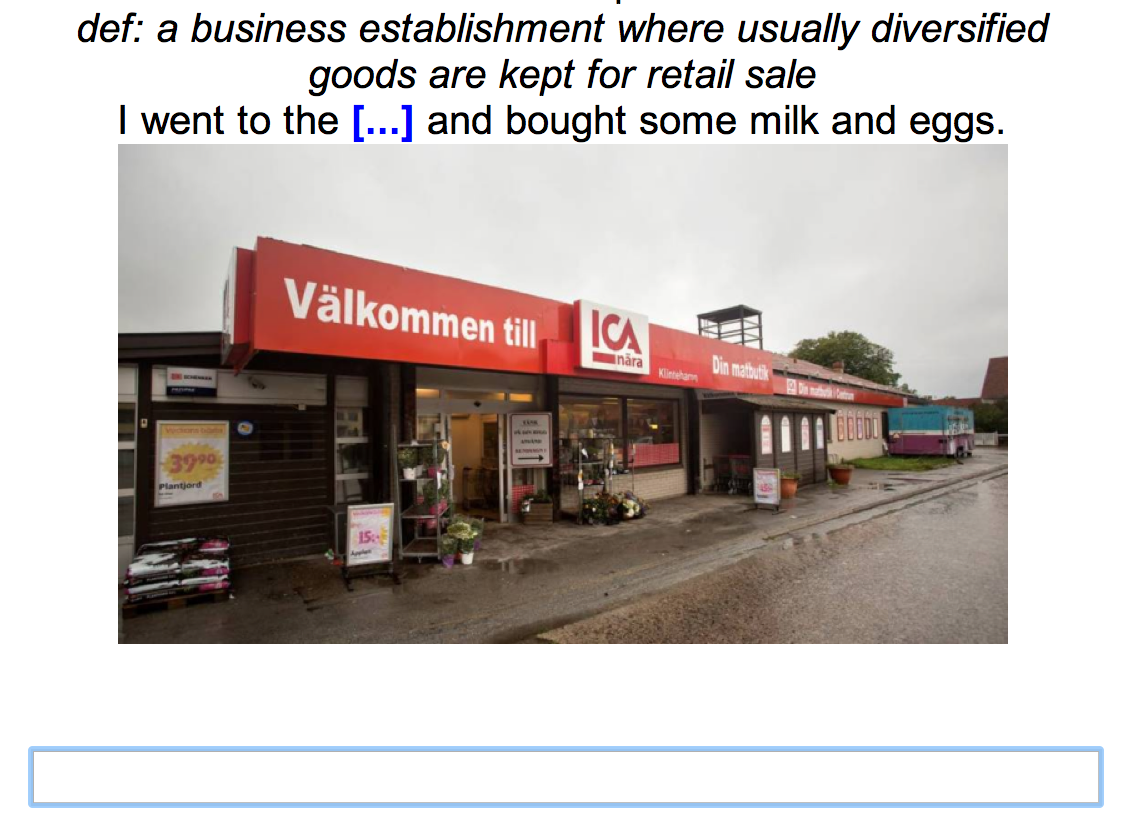
\includegraphics[scale=0.5]{cloze_example.png}
\caption{Anki Flashcard}
\label{fig:flashcard}
\end{figure}

After using this method of studying for some time, I have found that certain sentences work better than other for remembering new vocabulary and grammar.
Long sentences tended to be difficult to remember and were not as useful as I would tend to only look at a few words around the missing word.
Cards that had a personal association were much easier to recall.
Good definitions (simple and short but descriptive) helped as well.

In this paper I explore various machine learning approaches to predicting cloze deletion sentences from two Swedish news sources.
The goals for this paper were to answer the following questions:
\begin{itemize}
    \item Can we predict missing word using only the words around it?
    \item What sentences are good example sentences?
        \begin{itemize}
            \item Does length of sentence make a difference?
        \end{itemize}
    \item Where are good sources to find cloze deletion sentences?
\end{itemize}

I compare the difference between an LSTM (Long-Short term memory) neural network with that of a Bidirectional LSTM.
Later the two news sources (described in Section~\ref{sec:datasets}) are compared to see which data set is easier to predict.
Then I explore tuning the dropout parameter to see how overfitting can be improved.
Finally the predictions are analyzed to see which sentences are easy to predict.

\section{Data Sets} \label{sec:datasets}

\begin{figure}[h!]
\centering
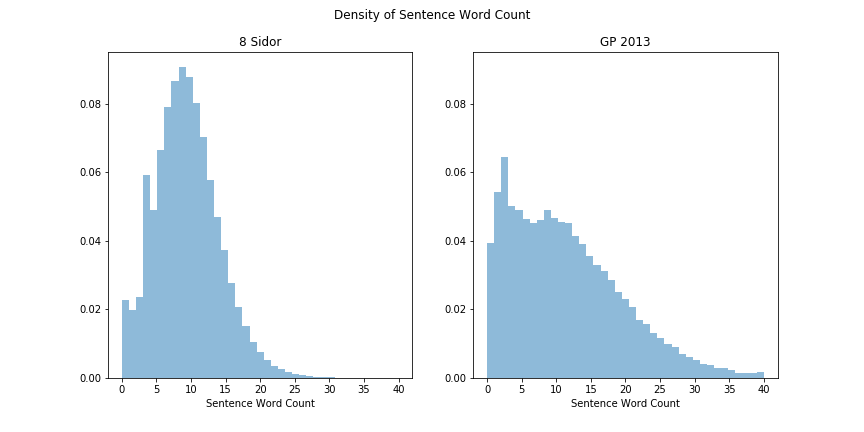
\includegraphics[scale=0.5]{word_count_density.png}
\caption{Sentence Word Count Density for 8 Sidor and Göteborgs-Posten 2013}
\label{fig:word_density}
\end{figure}

The data from Språkbanken comes in XML form  \cite{spraakbanken}.
The two data sets I compared were 8 Sidor (from 2002/11/14 to 2017/10/09) and Göteborgs-Posten (from 2013).
8 Sidor and Göteborgs-Posten differ in their goals as news sites.
8 Sidor describe itself on its website as "en nyhetstidning på lättläst svenska." \cite{8sidor}, which means that it is a newspaper in easy to read Swedish.
We can see this reflected in Table \ref{tab:possum} on page \pageref{tab:possum}.
Göteborgs-Posten (GP) is a more traditional \say{daily newspaper published in Gothenburg, Sweden} \cite{wiki:gp}.
Example sentence from the two 8 Sidor is, 

\begin{displayquote}
\say{Julian Assange säger att han kan gå med på att komma till Sverige och träffa svenska poliser.}
\end{displayquote}

and an example from Göteborgs-Posten is

\begin{displayquote}
\say{I morgon är det ett år sedan Wikileaks-grundaren	Julian Assange	klev in på Ecuadors ambassad i London på flykt undan de svenska brottsutredarna.}
\end{displayquote}

We can see from this example that Göteborgs-Posten uses more complex sentence structures and more advanced vocabulary.
This is also reflected in the word count usage as seen in Figure~\ref{fig:word_density}.
Göteborgs-Posten has a higher density of sentences with more words.
In general, longer sentences are often more complex grammatically.


\begin{table}[]
\centering
\begin{tabular}{lll}
\hline
& GP2013 & 8Sidor        \\ \hline
JJ     & 35377  & 4661  \\
VB     & 42729  & 9215  \\
NN     & 291292 & 39844 \\ \hline
\end{tabular}
\caption{Part-of-speech Count Summary} \label{tab:possum}
\end{table}

\section{Data Processing}

For exploration of the data, the Göteborgs-Posten -- Två Dagar (Two Days) data set was use which is a smaller example to start with.
The data set contains scrambled sentences from various text issues which are tagged with an issue id.
The first step was to build a data set with the raw sentence.
Python's built in XML package was for this step.
Sentences were joined from the \textit{w} (word) tags and part of speech tags were retained as well.
There were occasionally multiple sentences that were found in the same text tag.
These were kept as separate sentences at first but could be joined.
Punctuation was also removed from the sentences.
The available fields from Språkbanken data sets can be seen in Table~\ref{tab:spraakbankmeta}.

\begin{table}[h!]
\centering
\begin{tabular}{ll}
\hline
Ordattribut (id) & Lokalisering: svenska \\ \hline
word             & ord                   \\
pos              & ordklass              \\
msd              & msd                   \\
lemma            & saknas                \\
lex              & Lemgram               \\
sense            & betydelse             \\
prefix           & förled                \\
suffix           & efterled              \\
compwf           & sammansatta ordformer \\
complemgram      & sammansatta lemgram   \\
ref              & ref                   \\
dephead          & dephead               \\
deprel           & dependensrelation     \\ \hline
\end{tabular}
\caption{Språkbanken Metadata} \label{tab:spraakbankmeta}
\end{table}

For the analysis, the 8 Sidor data set was used (number of sentences was  $n = 254,711$).
Then, $n$ sentences were sampled from Göteborgs-Posten 2013.
This was done so that each data set had approximately the same number of sentences so that we can compare the results fairly.

% Reservoir Sampling was used to sample from the Göteborgs-Posten data set \cite{reservoir}. The idea behind reservoir sampling is that we want to get a sample of size $k$ from a data set without knowing $n$, the total number of elements. This is useful for this application because the GP2013 data set is very large. The first $k$ sentences are taken from the data set. Then for each $i = k + 1$ to $n$, we take a random integer $j, 1 \leq j \leq k$. If $i \leq j$, then we replace index $j$ with this new sentence.

\subsection{Creating Training Examples} \label{data_processing}
Each sentence is divided into potentially many training examples. 
For each noun, adjective, or verb in a sentence a window around the word was selected.
If we let define the window $k$, and a sentence is defined as $s = (w_0,\ldots, w_n)$ where $w_i$ is a word in the sentence (excluding punctuation).
Then for a word $w_i$, we use $(w_{i-k},\ldots,w_{i-1},w_{i+1},\ldots,w_{i + k})$ to try to predict $w_i$.
The before window is pre-padded with zeros when there are not three words found before the target word.
The after window is post-padded with zeros.
For all of the experiments a window size of 3 was used to predict the words.

\section{Comparing LSTM and Bidirectional LSTM}
The first experiment I ran was to compare the results of a standard LSTM and Bidirection LSTM.
Keras is used to create the neural networks in this paper \cite{keras}.
The hypothesis was that a bidirectional LSTM would provide better results because of the natural forward and backward context for the word.
For example, compare the two sentence below that have the same start but end very differently.
As seen in Figure~\ref{fig:rnn_brnn}, the standard LSTM feeds the sequence in in one direction and does not have access to the later data. The bidirectional feeds in both directions which allows for seeing the future data.

\begin{displayquote}
I went to the $\rule{1cm}{0.15mm}$ and bought some milk and eggs.
\end{displayquote}

\begin{displayquote}
I went to the $\rule{1cm}{0.15mm}$ and swam 10 laps.
\end{displayquote}

Using a bidirectional LSTM will allow the model to use the information from later in the sequence which could potentially improve the performance on sentences like this example. \cite{ngcoursera}

\begin{figure}[h!]
\centering
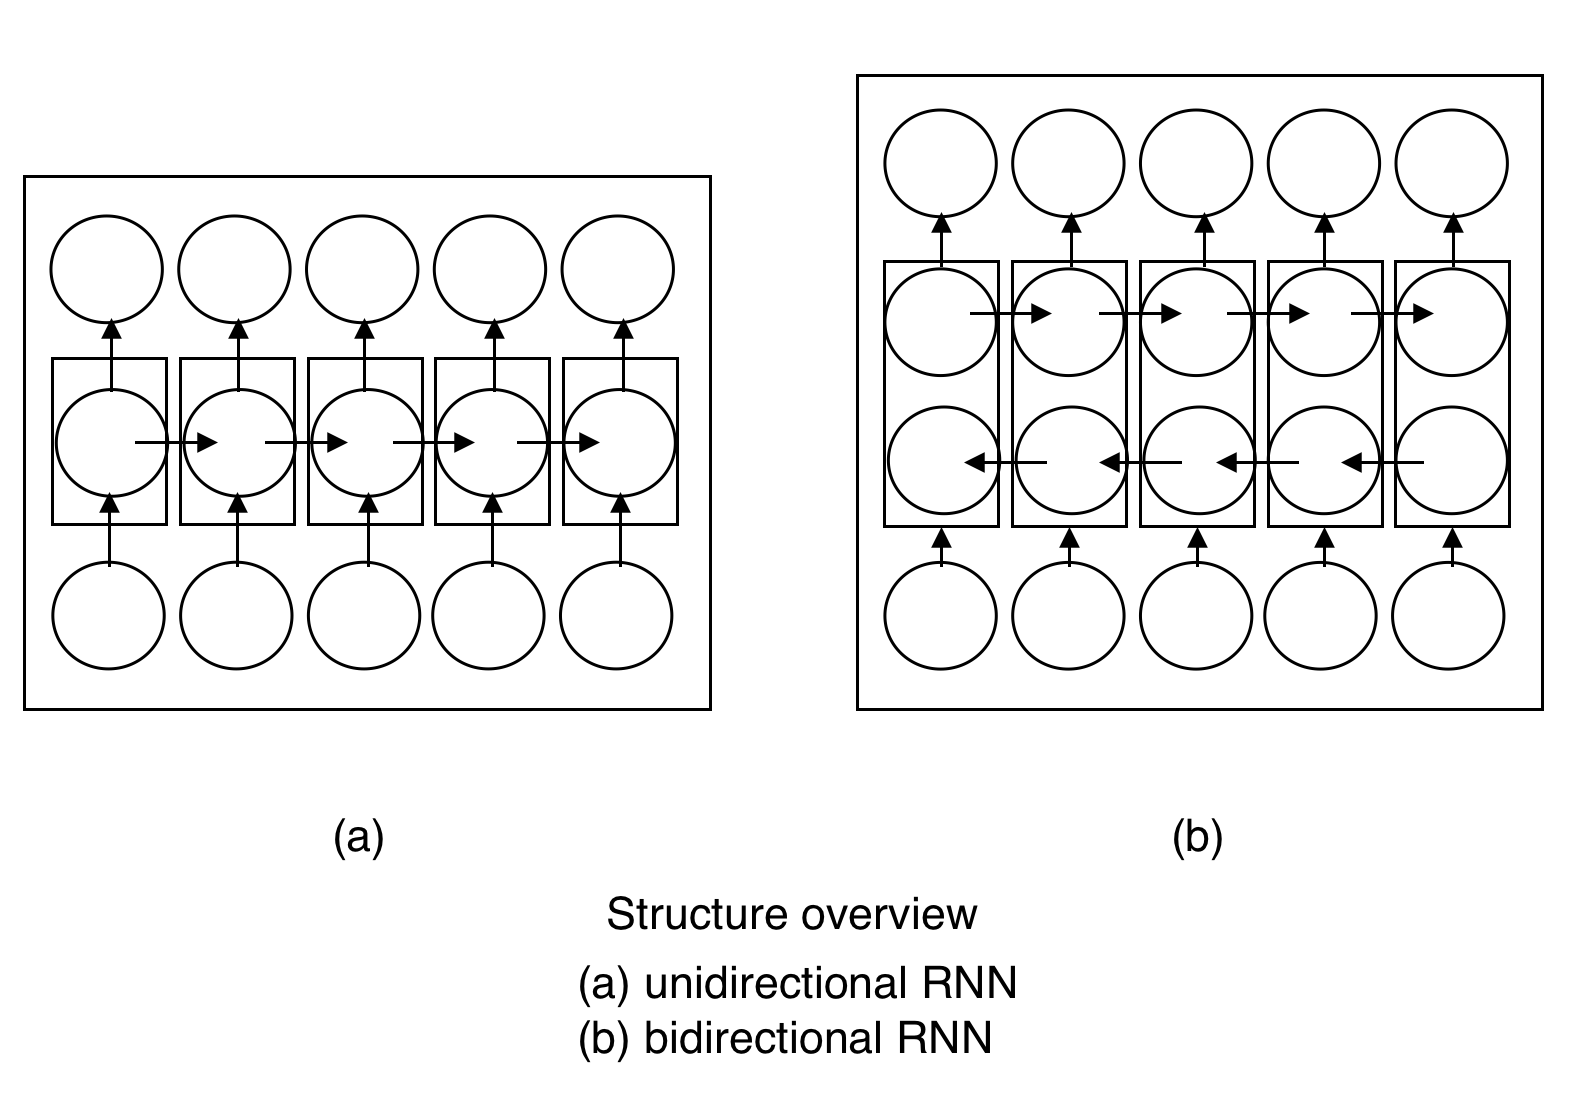
\includegraphics[scale=0.4]{RNN_BRNN.png}
\caption{RNN compared with Bidirectional RNN \cite{brnn}}
\label{fig:rnn_brnn}
\end{figure}

\subsection{Model Configuration} \label{sec:model_config}
For the first test, the 8 Sidor data set was used (number of sentences was  $259,216$.)
A 30\% validation set was used which resulted in $202,687$ validation samples.
Keras was used to implement the neural network \cite{keras}.
A window size of 3 was used with $10,000$ word limit on the vocabulary.
Only verbs, adjectives, and nouns were used as the prediction word.
Any word out of vocabulary was replaced with \textit{UNK}, and if the out of vocabulary word was found in either the before window, the word, or the after window the training example was discarded.
This resulted in $472,934$ training examples.

\begin{figure}[h!]
\centering
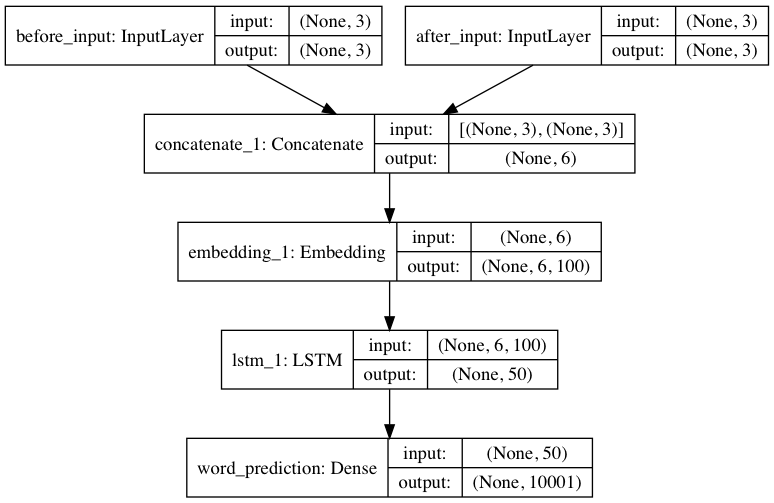
\includegraphics[scale=0.3]{atta_sample_lstm.png}
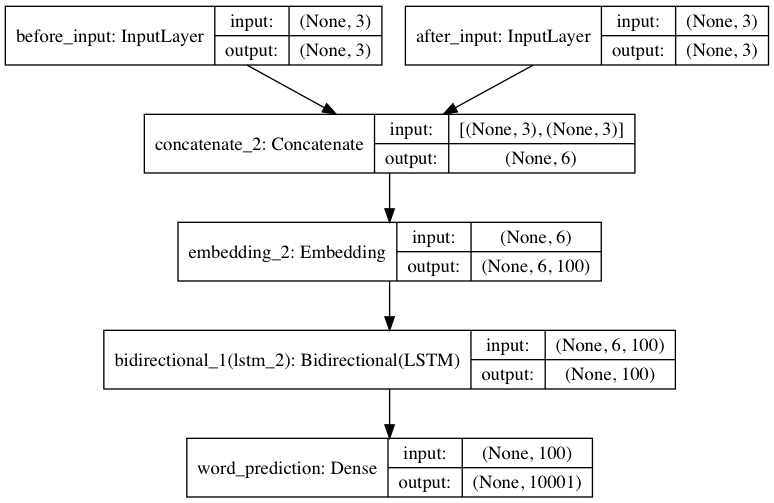
\includegraphics[scale=0.3]{atta_sample_blstm.png}
\caption{LSTM and Bidirectional LSTM Models}
\label{fig:compare_lstm}
\end{figure}

The models were identical apart from the LSTM layer being bidirectional which can be seen in Figure \ref{fig:compare_lstm}.
The before window and after window are first concatenated into a single layer.
Then an embedding layer is used with an embedding size of 100.
The LSTM layer has 50 units, with the default Keras parameters of activation being $tanh$.
There is a dropout of $0.1$ on both of the LSTM layers.
The output layer has dimension $10,000 + 1$ (the additional $+1$ is to include the out of vocabulary token), with a softmax activation.
The models were trained with the \textit{Adam} optimizer with 30 epochs and batch size 64.
The loss function is categorical cross entropy.
The categorical cross entropy is a sum of each of the individual cross entropy results for each category \cite{wiki:crossentropy}.
$$
H(y, \hat{y}) - \frac{1}{n} \sum_{i = 1}^{n} \sum_{j = 1}^{m} y_{i,j} \log(\hat{y}_{i,j})
$$
Where $y$ is a vector of the true values, and $\hat{y}$ are our predictions.
We define $n$ as the number of examples, $m$ as the number of categories and $y_{i,j}$ as the $i$th example with category $j$.
We only have one non-zero value of $y_{i,j}$ for each $i$.
So we can re-write this as
$$
H(y, \hat{y}) - \frac{1}{n} \sum_{i = 1}^{n} y_{i,c} \log(\hat{y}_{i,c})
$$
where $c$ is the only non-zero category for training example $i$ since we do not have more than one category.

\subsection{Results}

\begin{figure}[h!]
\centering
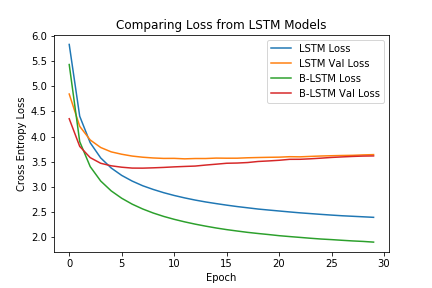
\includegraphics[scale=0.5]{blstm_compare_loss.png}
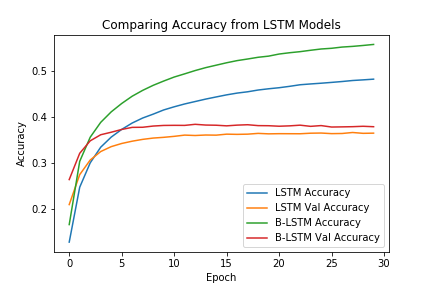
\includegraphics[scale=0.5]{blstm_compare_acc.png}
\caption{Comparing accuracy and cross-entropy loss between LSTM and Bidirectional LSTM Models}
\label{fig:lstm_compare_loss}
\end{figure}

Figure \ref{fig:lstm_compare_loss} shows the accuracy and the categorical cross entropy for the LSTM and the Bidirectional LSTM model.
We can see the Bidirectional LSTM model performs much better than the LSTM model on the training data.
It also performs a little bit better on the validation data.
From these plots we can see that both the models are over fitting but the Bidirectional LSTM model is over fitting more so than the standard LSTM model.

\section{Improving Overfitting}
One way to reduce overfitting is to use dropout.
Dropout removes random nodes from a neural network while training to prevent the network from learning too much from the noise in the dataset \cite{dropout_srivastava}.
In the LSTM and Bidirectional LSTM comparison a dropout of $0.1$ was used for the inputs to the LSTM.
To combat overfitting, the Bidirectional LSTM model model was compared with dropout rates $0.2$

\subsection{Dropout Comparison}

\begin{figure}[h!]
\centering
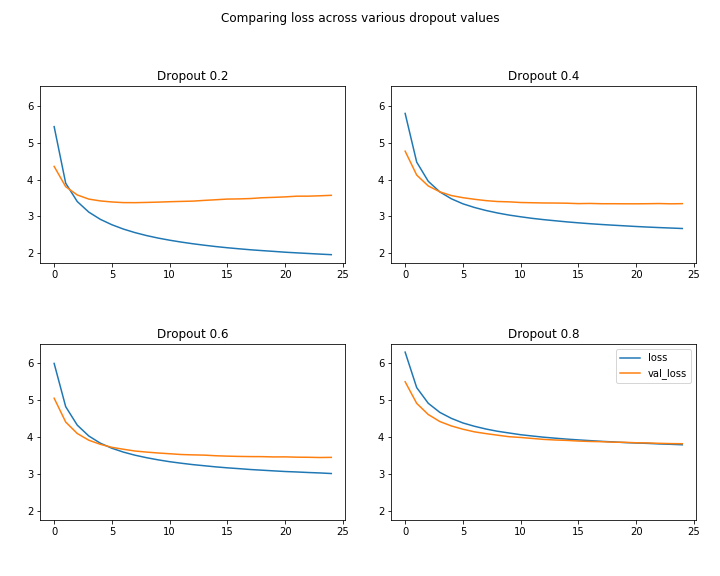
\includegraphics[scale=0.65]{dropout_compare_plot.png}
\caption{Comparing dropout values of 0.2, 0.4, 0.6 and 0.8 on Bidirectional LSTM Model}
\label{fig:dropout_compare_loss}
\end{figure}

Using the Bidirectional LSTM model described in Section~\ref{sec:model_config}, an experiment was set up to see how dropout parameter affected the results on the model.
All models has the Bidirectional LSTM Layer configured with the dropout set to the value $d = 0.2, 0.4, 0.6, 0.8$.
The models were all run with 25 epochs ($0,\ldots,24$) that took about 300 seconds for each epoch.
The recurrent dropout is also set to the same $d$ value.
As described in \cite{recurrent_dropout}, the recurrent dropout randomly drops recurrent connection within the LSTM.
The normal dropout parameter randomly drops the inputs and output into and out of the LSTM layer.

\begin{table}[h!]
    \centering
    \begin{tabular}{rrr}
    \toprule
     Dropout &  Minimum Loss &  Minimum Loss Epoch \\
    \midrule
         0.2 &         3.374 &                   7 \\
         0.4 &         3.342 &                  23 \\
         0.6 &         3.451 &                  23 \\
         0.8 &         3.824 &                  24 \\
    \bottomrule
    \end{tabular}
    \caption{Comparing minimum loss across different dropout parameters} \label{tab:dropout_loss}
\end{table}

We can see that with dropout set to $0.2$, that the difference between the validation loss and the training loss is very high.
The validation loss also starts to increase after epoch 7.
The minimum value achieve was at epoch 7, with a categorical cross entropy of 3.374.
For the other dropout values 0.4, 0.6, and 0.8 the minimum loss was 3.342, 3.451, and 3.824.
The results are summarized in Table~\ref{tab:dropout_loss} on page \pageref{tab:dropout_loss}.

We can see as the dropout value increases, the training loss and validation loss are closer together, indicating less overfitting.
When using a higher value of dropout, the model tends to converge slower.
That is, we need more epochs to reach the same loss level.
Both dropout of $0.6$ and $0.8$, but especially dropout of $0.8$ could have been run for much longer to see where the loss converges to.

\section{Prediction Analysis}
The model we trained on 8 Sidor data was used to find sentences that the model predicted very well.
First the model was used to predict the missing values.
Then the cross entropy was computed for each training example.

Figure \ref{fig:word_count_entropy} shows the average (mean) cross entropy for each word count group.
The points $(x,y)$ represent the mean cross entropy of each sentence that has a word count of $x$.
The bars represent the standard deviation within the each word count group.
We can see from this graph that very short sentences are hard to predict ($x < 5$) as well as large sentences ($x > 25$).


\begin{figure}[h!]
\centering
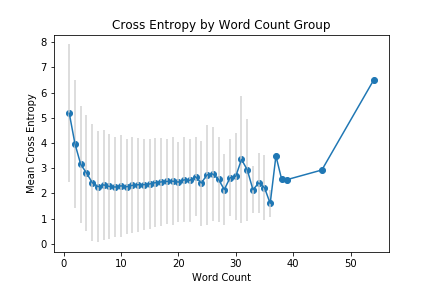
\includegraphics[scale=1]{cross_entropy_word_count.png}
\caption{Average Cross Entropy for each word count group}
\label{fig:word_count_entropy}
\end{figure}

\subsection{Best Prediction Examples}

\begin{table}[h!]
\centering
\begin{tabular}{l p{10cm}}
\toprule
   Word &                                                                                                              Sentence \\
\midrule
 initiativ &  Partiet Feministiskt initiativ ställer upp i valet till EUs riksdag , Europaparlamentet . \\
 eurovision &  Sanna Nielsen från Sverige sjöng i musiktävlingen Eurovision Song Contest , ESC , på tisdagen . \\
 champions &  Malmö FF förlorade även den andra matchen mot Juventus i Champions League i fotboll . \\
 fredspris &  Liu Xiaobo från Kina får Nobels fredspris i år . \\
 eld &  Men muslimska ledare tror att någon tänt eld på huset . \\
 tv &  Rättegången kommer att sändas i TV 4 plus . \\
 bin &  Usama bin Ladin är \\
 förenta &  Förenta Nationernas organisation Barnfonden säger att det finns sextusen barnsoldater i Sudan i Afrika . \\
 green &  Höjdhopparen Emma Green Tregaro har också en bra chans att ta medalj . \\
 sos &  Emil ringde till SOS Alarm för att bli hämtad av en ambulans . \\
 för &  Centrum för lättläst får pengar av staten för att göra det . \\
 vicepresident &  Det säger USAs vicepresident Joe Biden . \\
 real &  Kampen står mellan Ronaldo från Real Madrid och Lionel Messi eller Andres Iniesta från Barcelona , tror experterna . \\
 daglig &  Daglig verksamhet är inte ett jobb som du får lön för att göra . \\
 röda &  Men nu stoppar både Röda Korset och FN hjälpen till de människor som är fast i Aleppo . \\
 fängelse &  Han är misstänkt för spioneri och kan dömas till livstids fängelse i USA . \\
 procent &  Bland eleverna är Miljöpartiet tredje största parti med nästan 15 procent av rösterna . \\
 meter &  Susanna Kallur vann 100 meter häck vid en gala i Karlstad på onsdagen . \\
 butikskedjan &  Fabian Bengtsson är chef för butikskedjan Siba som säljer elektronik . \\
 alarm &  Företaget SOS Alarm har fått hård kritik den senaste tiden . \\
\bottomrule
\end{tabular}
\caption{Best prediction examples for 8 Sidor data set}\label{tab:pred_examples}
\end{table}

In Table~\ref{tab:pred_examples} on page \pageref{tab:pred_examples}, we can see the predictions from the model which had the lowest cross entropy.
Many of these top predicted words are parts of proper nouns or named entities which is fairly obvious because these words don't appear in other contexts on their own.

Some notable example from this list that would be good cloze deletion example are: \textit{initiativ, eld, fängelse, procent, meter}.
\begin{itemize}
    \item Partiet Feministiskt \textbf{initiativ} ställer upp i valet till EUs riksdag, Europaparlamentet.
    \item Men muslimska ledare tror att någon tänt \textbf{eld} på huset. (Good in the sense that \say{tända eld (på)} goes together frequently)
    \item Han är misstänkt för spioneri och kan dömas till livstids \textbf{fängelse} i USA.
    \item Bland eleverna är Miljöpartiet tredje största parti med nästan 15 \textbf{procent} av rösterna.
    \item Susanna Kallur vann 100 \textbf{meter} häck vid en gala i Karlstad på onsdagen.
\end{itemize}

For future work, removing these named entities would potentially be better for a language learner.
We can also see from these example sentences that when named entities are found within the window that the predictions are very high.
For example, for predicting \textit{initiativ}, the proceeding words \textit{Partiet Feministiskt} are likely not seen anywhere else in the data set.
These type of examples can be good for a learner that has a connection in some way to \textit{Partiet Feministiskt}, to learn the word for \textit{initiativ}. 
\section{Comparing GP2013 and 8 Sidor}
To create a fair comparison, a tokenizer was fit on the joined text from both data sets.
The GP2013 data set is an sample equal in size to the full 8 Sidor data set.
The vocabulary size was set to $10,000$.
For this comparison $n = 44,981$, validating on $19,278$.
The reason this number is so much smaller when training only on 8 Sidor data is that the vocabulary is now much larger.
As described in section \ref{data_processing}, the training examples are not used if there is an \textit{UNK} token found in the window or the prediction word.
Since the total number of words in the vocabulary is larger, there will be many more words excluded.
This results in a total smaller number of examples.
While this is a rather small amount of data it is the same for both data sets so we can compare the results between them.
The model is configured the same as described in \ref{sec:model_config}, but with dropout set to $0.2$.
The tokenizer was the same for each data set but the models are trained individually.
The data was fit with 30 epochs.

\subsection{Results}

\begin{figure}[h!]
\centering
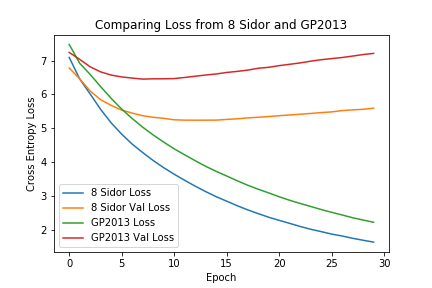
\includegraphics[scale=0.5]{compare_atta_gp_loss.png}
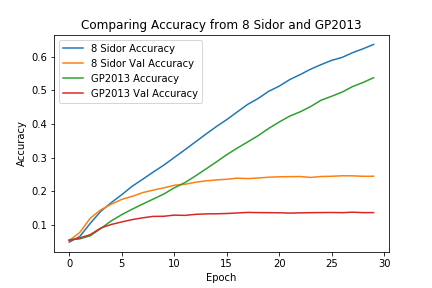
\includegraphics[scale=0.5]{compare_atta_gp_acc.png}
\caption{Comparing accuracy and cross-entropy loss between 8 Sidor and GP 2013}
\label{fig:atta_gp2013_compare}
\end{figure}

We can see in Figure~\ref{fig:atta_gp2013_compare} the cross entropy and the accuracy for each of the data sets. 
The training loss decreasing fast for both data sets.
As seen in section \ref{sec:model_config} the model overfits the training data.
The loss for the Göteborgs-Posten data set actually starts to increase with the number of epochs.
Overall, the model can predict better on the 8 Sidor data set than the data from Göteborgs-Posten 2013.

These results are consistent with the original hypothesis.
8 Sidor's intention is to create simple to read new articles without complicated sentence structure and words.
Often readers of this newspaper are learners of the Swedish language.
Göteborgs-Posten wants to be interesting to its audience, which has presumably a majority native Swedish speakers.
The writers want to write in an interesting way to convey a message with a much broader vocabulary.
This can be seen in the part of speech count summary found in Table~\ref{tab:possum} on page \pageref{tab:possum}.

\section{Conclusion}
In the paper I explored how we can predict cloze deletion sentences using recurrent (LSTM) neural networks.
The bidirectional variant of LSTM was compared with a standard LSTM model.
The dropout parameter was tuned through experiments on the 8 Sidor data set.

The top predicted example sentences showed that proper nouns and named entities were the easiest for the network to predict.
The length of the sentence did not play that much of a role, which is likely due to the window size selected.
We showed that when comparing Göteborgs-Posten and 8 Sidor that the neural network had an easier time predicting the sentences from 8 Sidor.
Using other preprocessing methods would be the greatest improvement to the process.

While the results were not great in predicting, there is much potential for improve the model and exploring cloze deletion in more detail.
Future work could include dictionary definitions as input the the neural network.
Other hyperparameters could be tuned to make the network predict better.
The training example creation stage could also be improved and filtering for named entities and proper noun would make the example sentences better.
Using other data sources than news sources would potentially give better example sentences.

\bibliographystyle{plain}
\bibliography{references}
\end{document}
